%%%%%%%%%%%%%%%%%%%%%%%%%%%%%%%%%%%%%%%%%
% Beamer Presentation
% LaTeX Template
% Version 1.0 (10/11/12)
%
% This template has been downloaded from:
% http://www.LaTeXTemplates.com
%
% License:
% CC BY-NC-SA 3.0 (http://creativecommons.org/licenses/by-nc-sa/3.0/)
%
%%%%%%%%%%%%%%%%%%%%%%%%%%%%%%%%%%%%%%%%%

%----------------------------------------------------------------------------------------
%	PACKAGES AND THEMES
%----------------------------------------------------------------------------------------

\documentclass[UTF8,aspectratio=169,12pt]{ctexbeamer}

\usepackage{hyperref}
\hypersetup{
	colorlinks=true,
	linkcolor=red,
	anchorcolor=blue,
	citecolor=green
}

\mode<presentation> {
	
	% The Beamer class comes with a number of default slide themes
	% which change the colors and layouts of slides. Below this is a list
	% of all the themes, uncomment each in turn to see what they look like.
	
	%\usetheme{default}
	%\usetheme{AnnArbor}
	%\usetheme{Antibes}
	%\usetheme{Bergen}
	%\usetheme{Berkeley}
	%\usetheme{Berlin}
	%\usetheme{Boadilla}
	%\usetheme{CambridgeUS}
	%\usetheme{Copenhagen}
	%\usetheme{Darmstadt}
	%\usetheme{Dresden}
	%\usetheme{Frankfurt}
	%\usetheme{Goettingen}
	%\usetheme{Hannover}
	%\usetheme{Ilmenau}
	%\usetheme{JuanLesPins}
	%\usetheme{Luebeck}
	\usetheme{Madrid}
	%\usetheme{Malmoe}
	%\usetheme{Marburg}
	%\usetheme{Montpellier}
	%\usetheme{PaloAlto}
	%\usetheme{Pittsburgh}
	%\usetheme{Rochester}
	%\usetheme{Singapore}
	%\usetheme{Szeged}
	%\usetheme{Warsaw}
	
	% As well as themes, the Beamer class has a number of color themes
	% for any slide theme. Uncomment each of these in turn to see how it
	% changes the colors of your current slide theme.
	
	%\usecolortheme{albatross}
	%\usecolortheme{beaver}
	%\usecolortheme{beetle}
	%\usecolortheme{crane}
	%\usecolortheme{dolphin}
	%\usecolortheme{dove}
	%\usecolortheme{fly}
	%\usecolortheme{lily}
	%\usecolortheme{orchid}
	%\usecolortheme{rose}
	%\usecolortheme{seagull}
	%\usecolortheme{seahorse}
	%\usecolortheme{whale}
	%\usecolortheme{wolverine}
	
	%\setbeamertemplate{footline} % To remove the footer line in all slides uncomment this line
	%\setbeamertemplate{footline}[page number] % To replace the footer line in all slides with a simple slide count uncomment this line
	
	%\setbeamertemplate{navigation symbols}{} % To remove the navigation symbols from the bottom of all slides uncomment this line
}

\usepackage{graphicx} % Allows including images
\graphicspath{{./figs/}}
\usepackage{booktabs} % Allows the use of \toprule, \midrule and \bottomrule in tables
\usepackage{longtable}
\usepackage{xcolor}
\usepackage{minted}
\usepackage{listings}
\lstset{numbers=left, %设置行号位置
	numberstyle=\tiny, %设置行号大小
	keywordstyle=\color{blue}, %设置关键字颜色
	commentstyle=\color[cmyk]{1,0,1,0}, %设置注释颜色
	frame=single, %设置边框格式
	escapeinside=``, %逃逸字符(1左面的键),用于显示中文
	%breaklines, %自动折行
	extendedchars=false, %解决代码跨页时,章节标题,页眉等汉字不显示的问题
	xleftmargin=2em,xrightmargin=2em, aboveskip=1em, %设置边距
	tabsize=4, %设置tab空格数
	showspaces=false %不显示空格
}
% Fonts
% \usepackage{libertine}
% \setmonofont{Courier}
%\setCJKsansfont[ItalicFont=Noto Serif CJK SC Black, BoldFont=Noto Sans CJK SC Black]{Noto Sans CJK SC}


%----------------------------------------------------------------------------------------
%   TITLE PAGE
%----------------------------------------------------------------------------------------

\title[第5讲]{第五讲:物理内存管理 - 非连续内存分配} % The short title appears at the bottom of every slide, the full title is only on the title page
\subtitle{第5节:RISC-V页映射机制}
\author{向勇、陈渝、李国良} % Your name
\institute[清华大学] % Your institution as it will appear on the bottom of every slide, may be shorthand to save space
{
清华大学计算机系 \\ % Your institution for the title page
\medskip
\textit{xyong,yuchen,liguoliang@tsinghua.edu.cn} % Your email address
}
\date{\today} % Date, can be changed to a custom date

\begin{document}

\begin{frame}
\titlepage % Print the title page as the first slide
\end{frame}

%----------------------------------------------------------------------------------------
\begin{frame}
\frametitle{提纲} % Table of contents slide, comment this block out to remove it
\tableofcontents % Throughout your presentation, if you choose to use \section{} and \subsection{} commands, these will automatically be printed on this slide as an overview of your presentation
\end{frame}

%----------------------------------------------------------------------------------------
%   PRESENTATION SLIDES
%----------------------------------------------------------------------------------------
%------------------------------------------------
\section{第5节 RISC-V页映射机制}% Sections can be created in order to organize your presentation into discrete blocks, all sections and subsections are automatically printed in the table of contents as an overview of the talk
%------------------------------------------------
\subsection{RISC-V页映射机制} % A subsection can be created just before a set of slides with a common theme to further break down your presentation into chunks


%------------------------------------------------
\begin{frame}[fragile,plain]   
	\frametitle{回顾}
	
	\begin{columns}
		
		\begin{column}{.5\textwidth}
			
			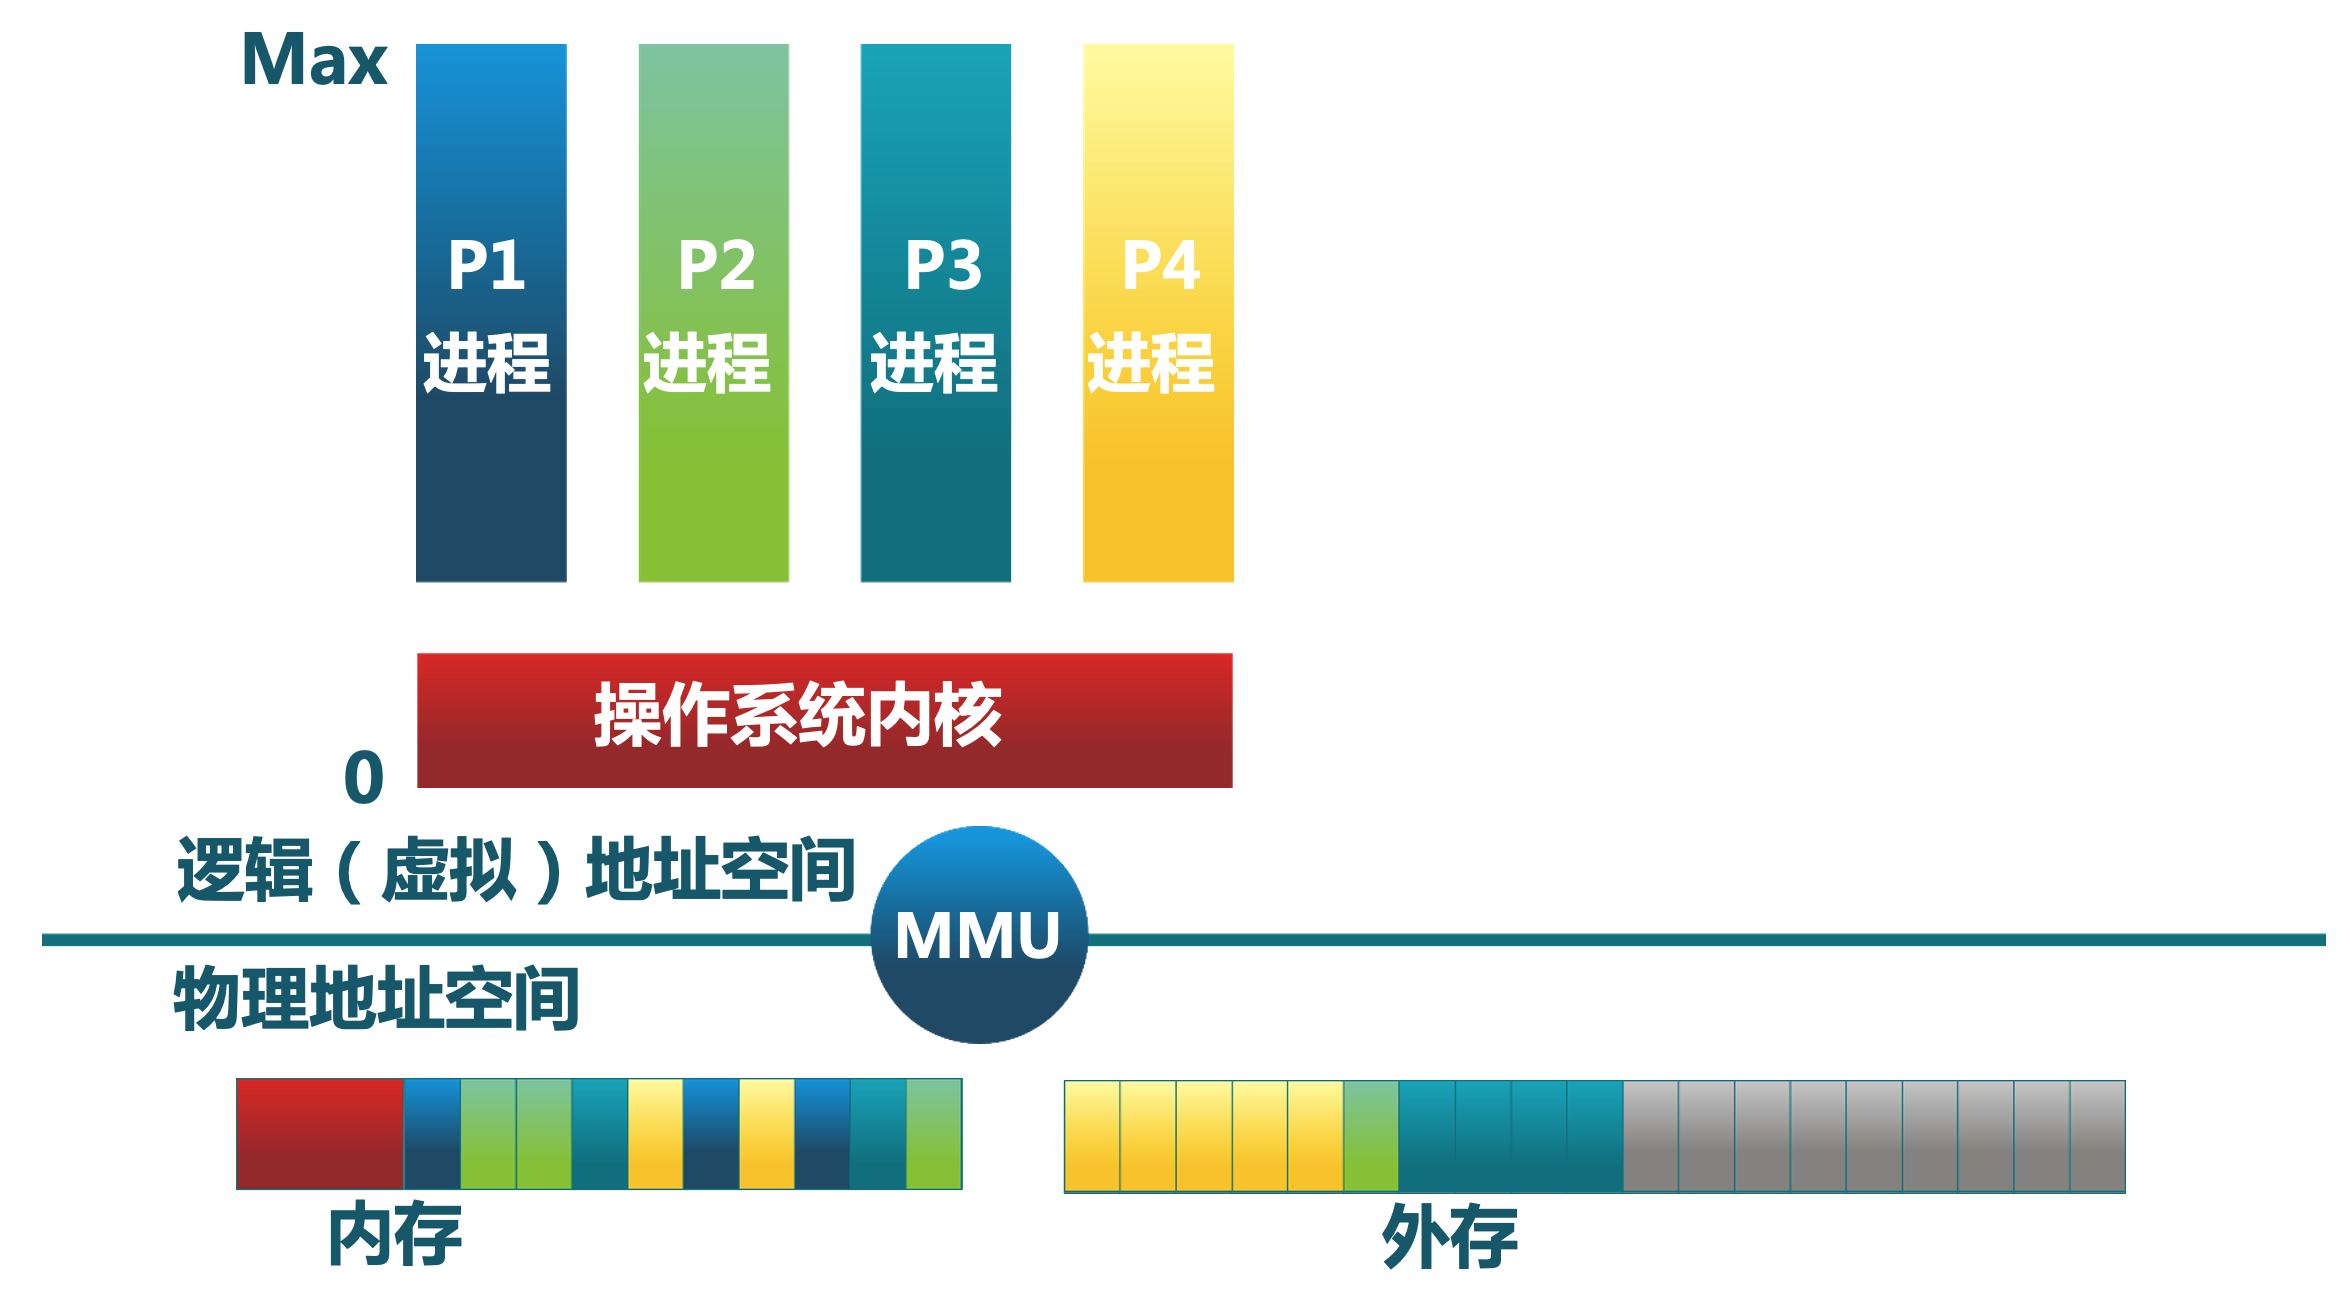
\includegraphics[width=1.2\textwidth]{mem-management}
			
		\end{column}
		
		
		\begin{column}{.5\textwidth}
			
			\begin{itemize}\large
				\item 通过页表来实现隔离与共享
				\begin{itemize}
					\item 运行的应用程序之间的隔离与共享
					\item 应用与内核之间的隔离与共享
					\item 便于非连续内存管理						
					\item RISC-V Privileged Architecture Version 1.10 (RV32/64)
					\item \href{http://crva.ict.ac.cn/documents/RISC-V-Reader-Chinese-v2p1.pdf}{The RISC-V Reader第10.6节}	
				\end{itemize}
			\end{itemize}
			\centering
			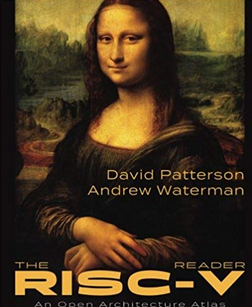
\includegraphics[width=.3\textwidth]{rv-reader-book}
		\end{column}
		
		
	\end{columns}
	
\end{frame}

%------------------------------------------------
\begin{frame}[fragile,plain]   
	\frametitle{RISC-V页映射机制}
	
	\begin{columns}[t]
		
		\begin{column}{.4\textwidth}
			
			\centering
			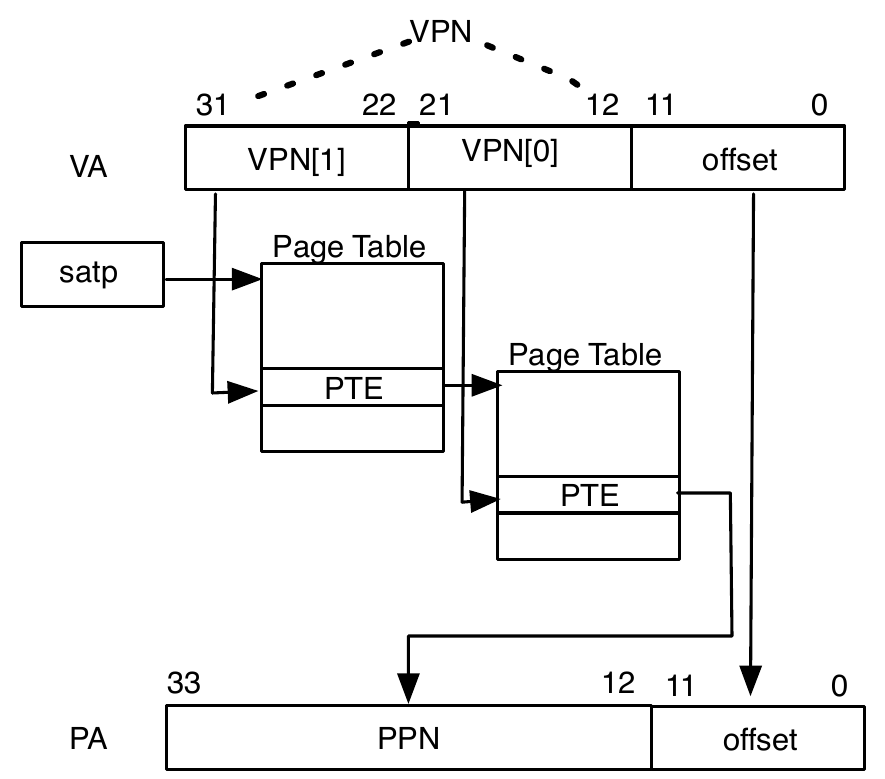
\includegraphics[width=.8\textwidth]{sv32-addr-trans}
			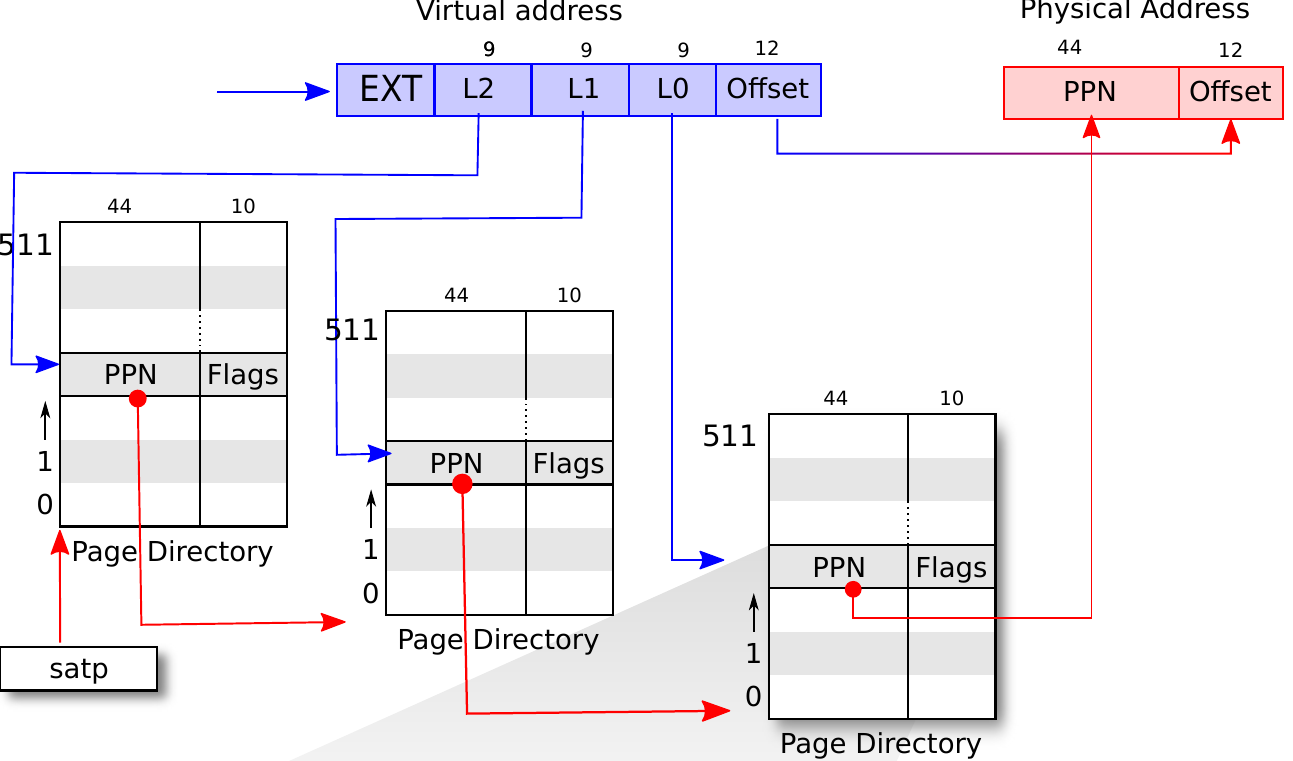
\includegraphics[width=.8\textwidth]{sv39-pagetable}
			
		\end{column}
		
		
		\begin{column}{.6\textwidth}
			
			\begin{itemize}\large
				\item RISC-V对页表的硬件支持
				\begin{itemize}
					\item RISC-V 32的Sv32虚地址与物理地址
					%					\item 
					
					
				\end{itemize}
			\end{itemize}
			
			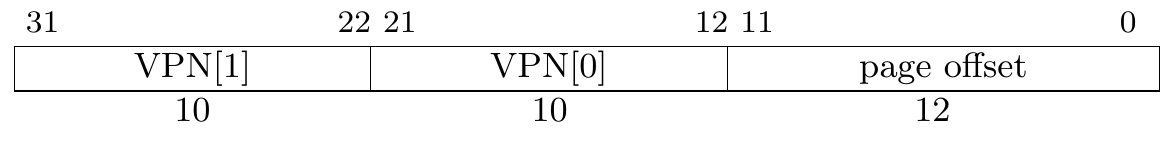
\includegraphics[width=1.\textwidth]{sv32va} \pause
			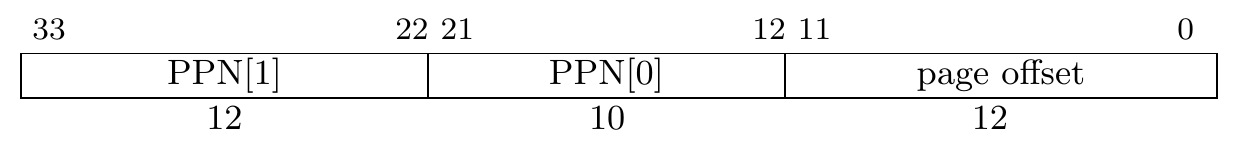
\includegraphics[width=1.\textwidth]{sv32pa}
			
		\end{column}
		
		
	\end{columns}
	
\end{frame}

%------------------------------------------------
\begin{frame}[fragile,plain]   
	\frametitle{RISC-V页映射机制}
	
	\begin{columns}[t]
		
		\begin{column}{.4\textwidth}
			
			\centering
			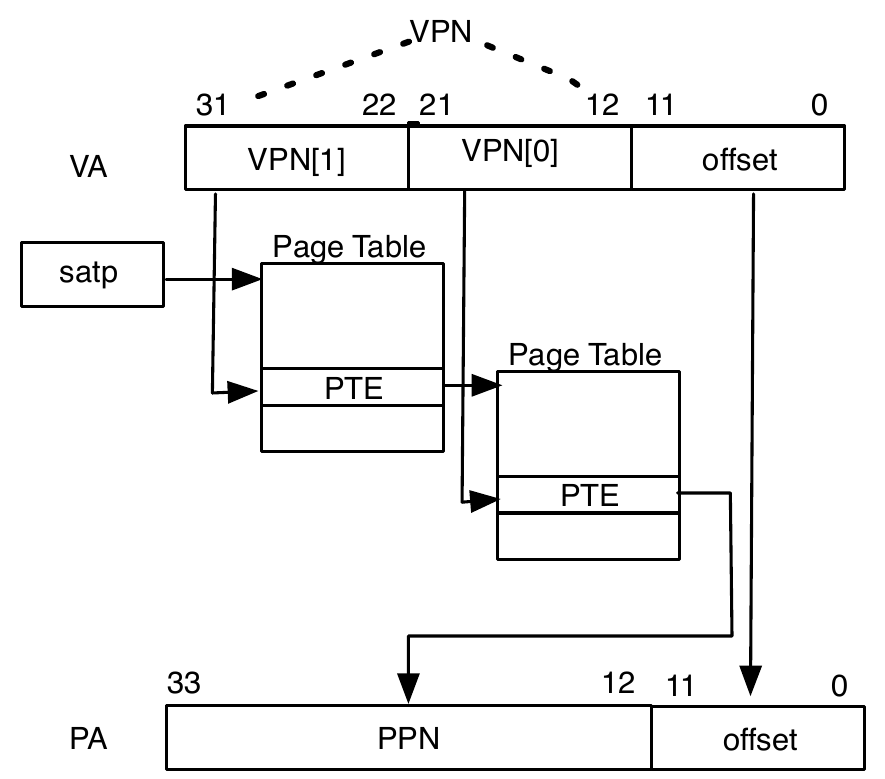
\includegraphics[width=.8\textwidth]{sv32-addr-trans}
			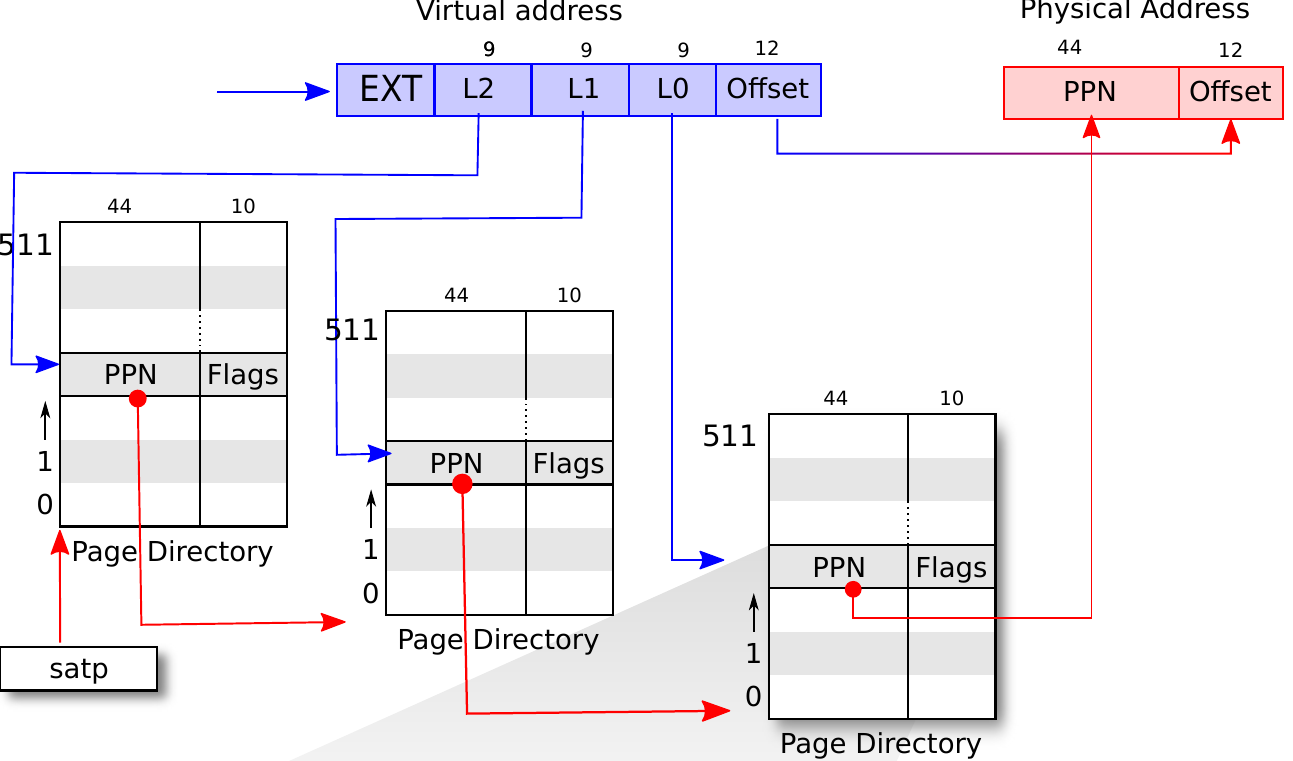
\includegraphics[width=.8\textwidth]{sv39-pagetable}
			
		\end{column}
		
		
		\begin{column}{.6\textwidth}
			
			\begin{itemize}\large
				\item RISC-V对页表的硬件支持
				\begin{itemize}
					\item RISC-V 64的Sv39虚地址与物理地址
%					\item 
					
					
				\end{itemize}
			\end{itemize}
			
			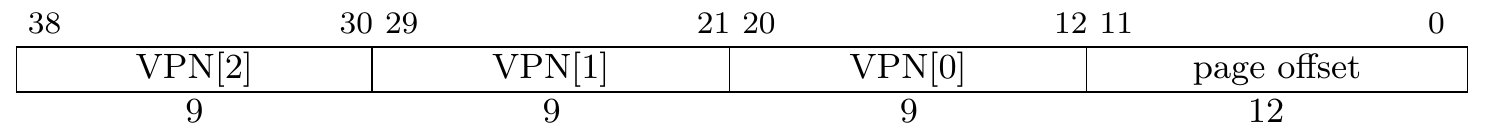
\includegraphics[width=1.\textwidth]{sv39va} \pause
			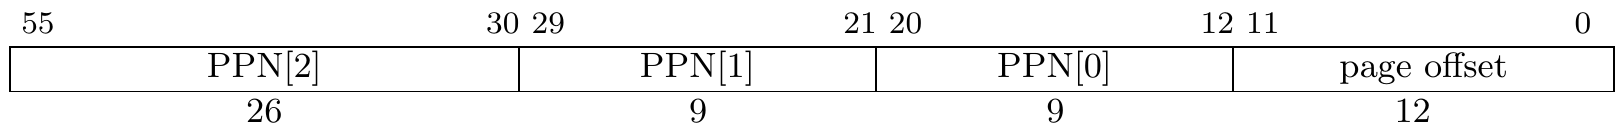
\includegraphics[width=1.\textwidth]{sv39pa}
			
		\end{column}
		
		
	\end{columns}
	
\end{frame}


%------------------------------------------------
\begin{frame}[fragile,plain]   
	\frametitle{RISC-V页映射机制}
	
	\begin{columns}[t]
		
		\begin{column}{.4\textwidth}
			
		\centering
		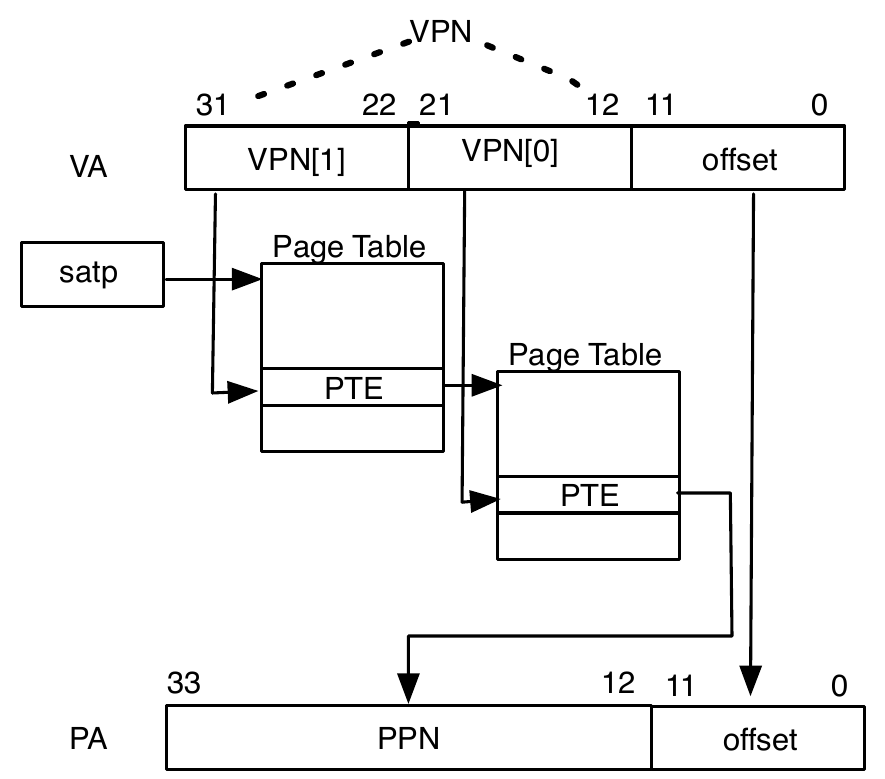
\includegraphics[width=.8\textwidth]{sv32-addr-trans}
		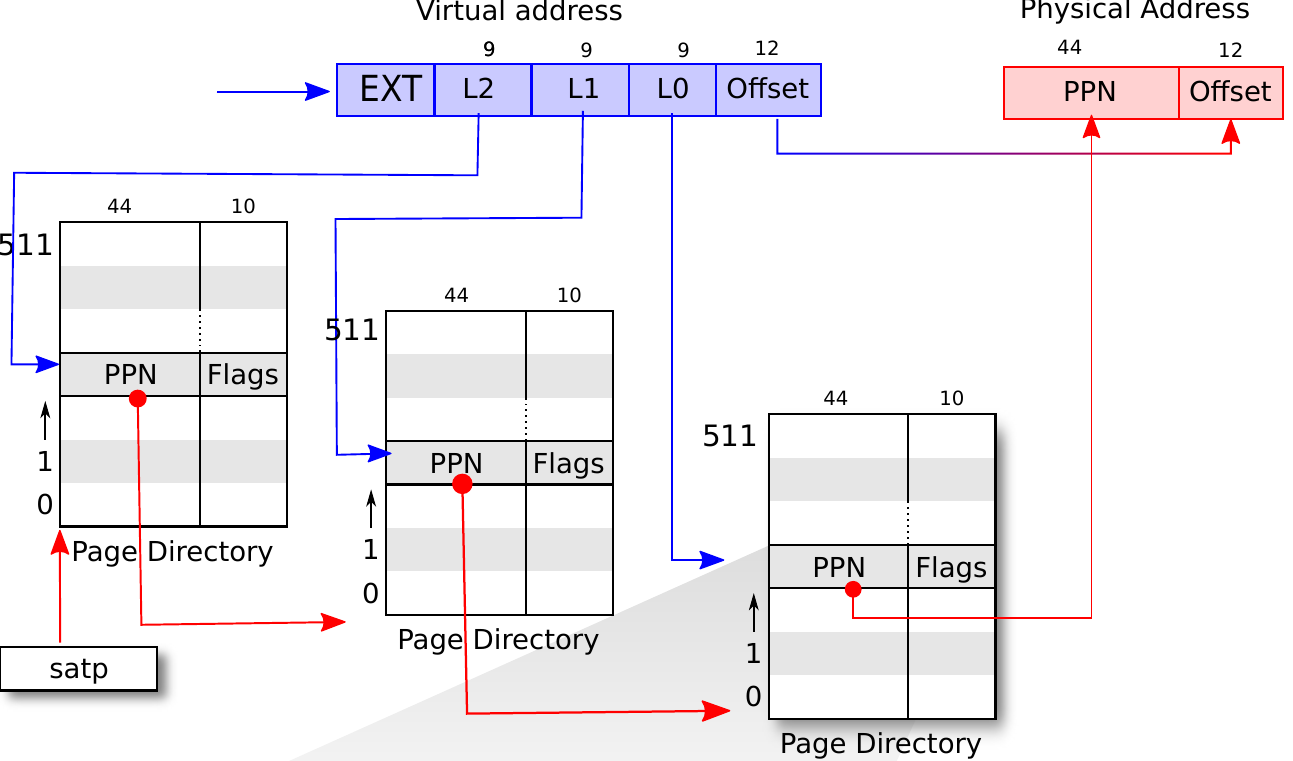
\includegraphics[width=.8\textwidth]{sv39-pagetable}
			
		\end{column}
		
		
		\begin{column}{.5\textwidth}
			
			\begin{itemize}\large
				\item RISC-V对页表的硬件支持
				\begin{itemize}
					\item 页表基址 \pause : satp in RISC-V 32
					\item  Supervisor Address Translation and Protection (satp) Register
					
							
				\end{itemize}
			\end{itemize}
			
			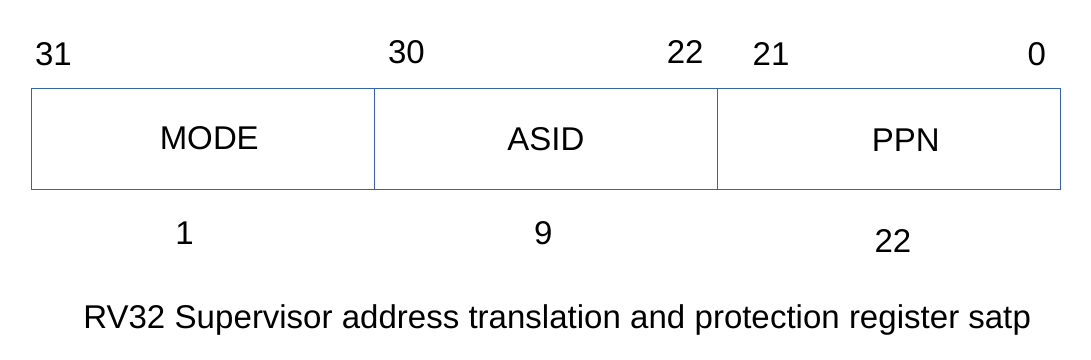
\includegraphics[width=1.\textwidth]{satp32}
%			\begin{figure}[h!]
%				{\footnotesize
%					\begin{center}
%						\begin{tabular}{c@{}E@{}K}
%							\instbit{31} &
%							\instbitrange{30}{22} &
%							\instbitrange{21}{0} \\
%							\hline
%							\multicolumn{1}{|c|}{{\tt MODE} (\warl)} &
%							\multicolumn{1}{|c|}{{\tt ASID} (\warl)} &
%							\multicolumn{1}{|c|}{{\tt PPN}  (\warl)} \\
%							\hline
%							1 & 9 & 22 \\
%						\end{tabular}
%					\end{center}
%				}
			
		\end{column}
		
		
	\end{columns}
	
\end{frame}


%------------------------------------------------
\begin{frame}[fragile,plain]   
	\frametitle{RISC-V页映射机制}
	
	\begin{columns}[t]
		
		\begin{column}{.4\textwidth}
	
	\centering
	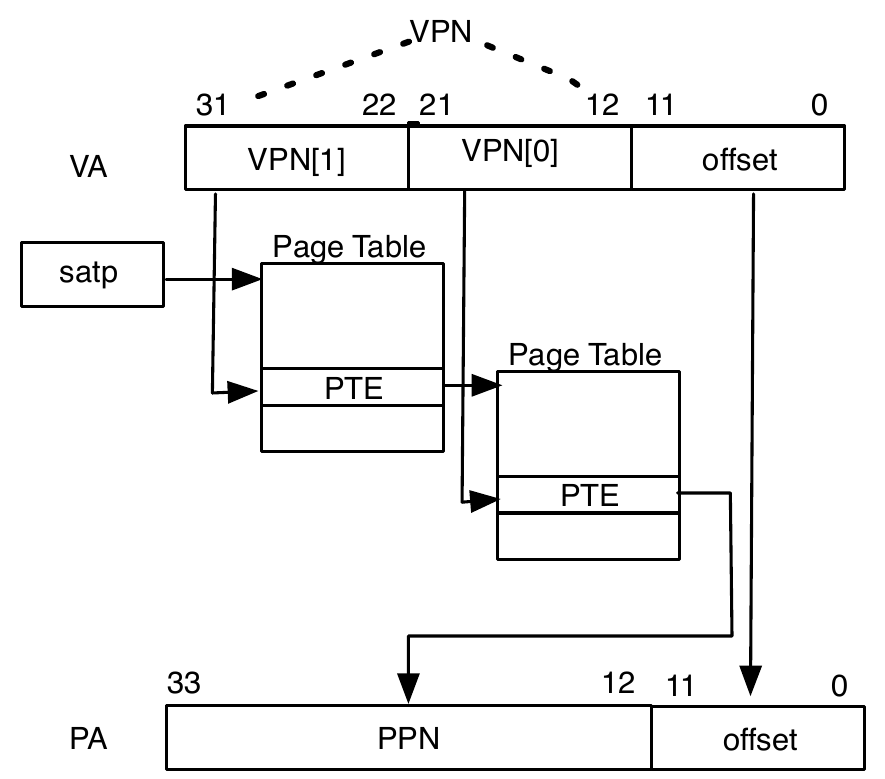
\includegraphics[width=.8\textwidth]{sv32-addr-trans}
	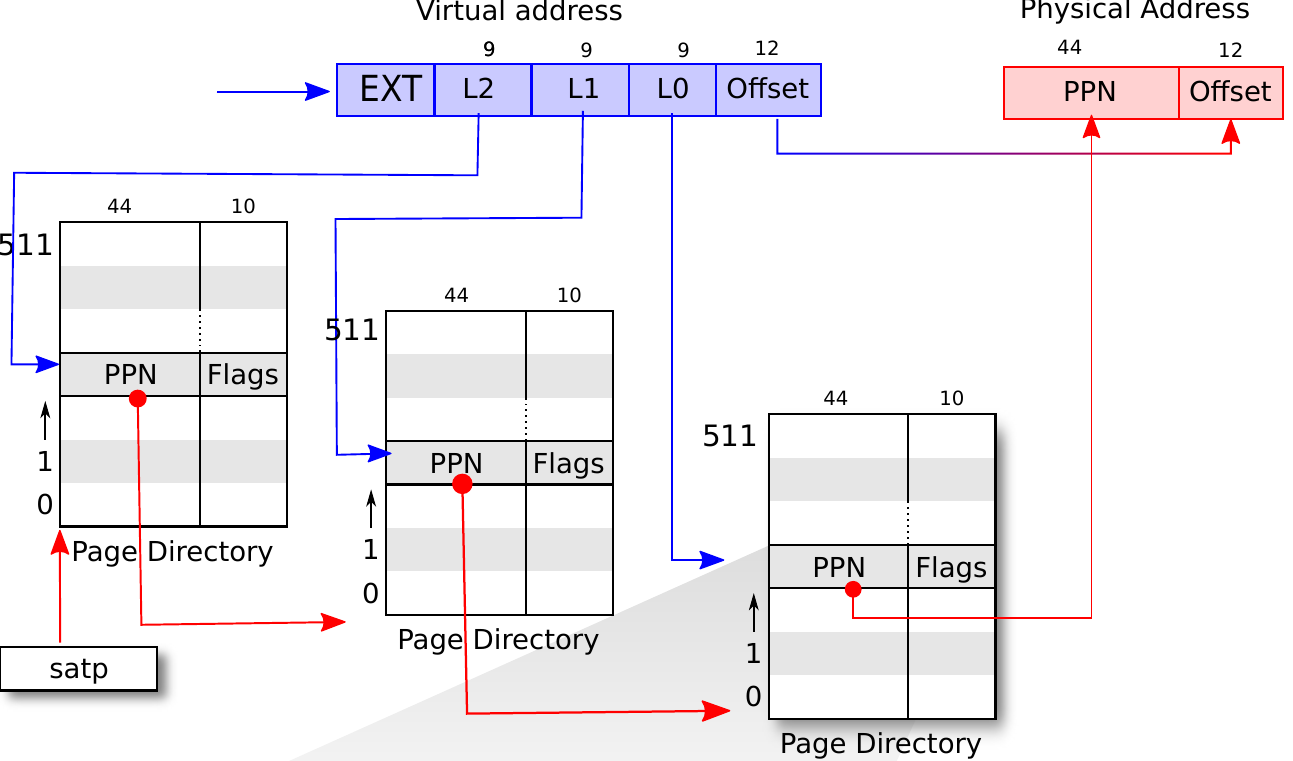
\includegraphics[width=.8\textwidth]{sv39-pagetable}
			
		\end{column}
		
		
		\begin{column}{.5\textwidth}
			
			\begin{itemize}\large
				\item RISC-V对页表的硬件支持
				\begin{itemize}
					\item 页表基址 : satp in RISC-V 64
					\item  Supervisor Address Translation and Protection (satp) Register
					
					
				\end{itemize}
			\end{itemize}
             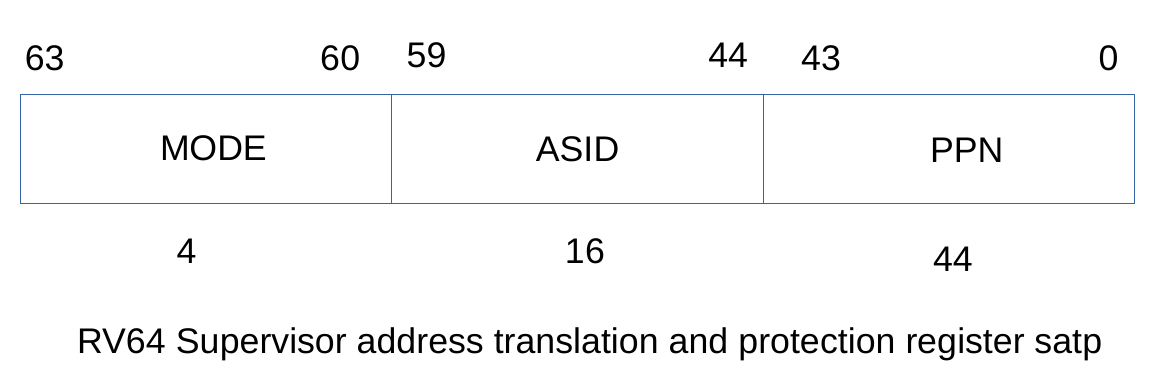
\includegraphics[width=1.\textwidth]{satp64}
		\end{column}
		
		
	\end{columns}
	
\end{frame}


%------------------------------------------------
\begin{frame}[fragile,plain]   
	\frametitle{RISC-V页映射机制}
	
	\begin{columns}[t]
		
		\begin{column}{.5\textwidth}
			
			\centering
			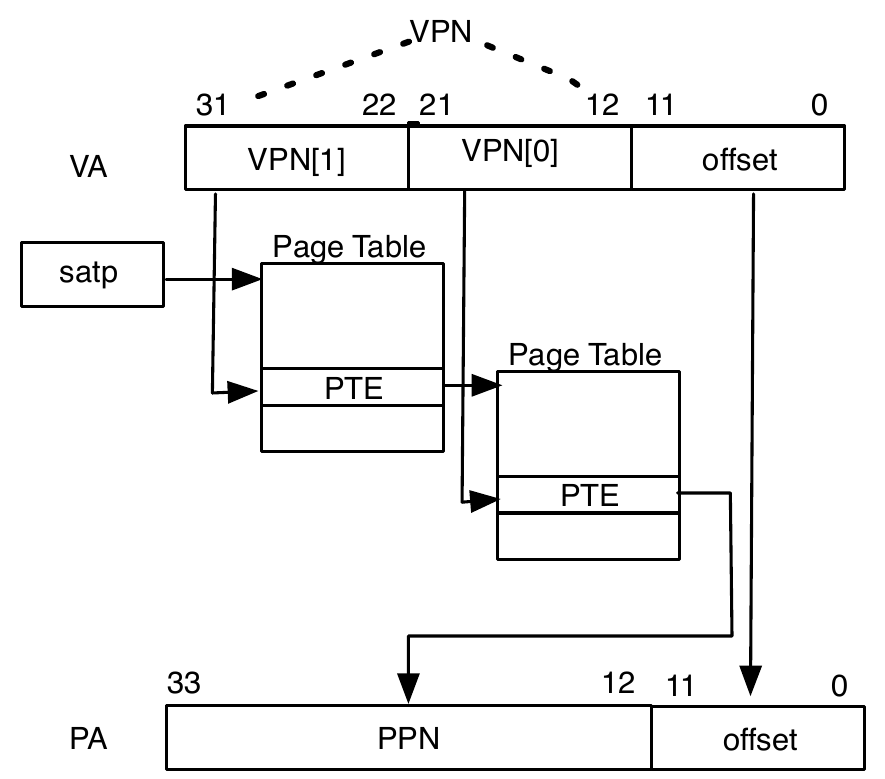
\includegraphics[width=.6\textwidth]{sv32-addr-trans}
			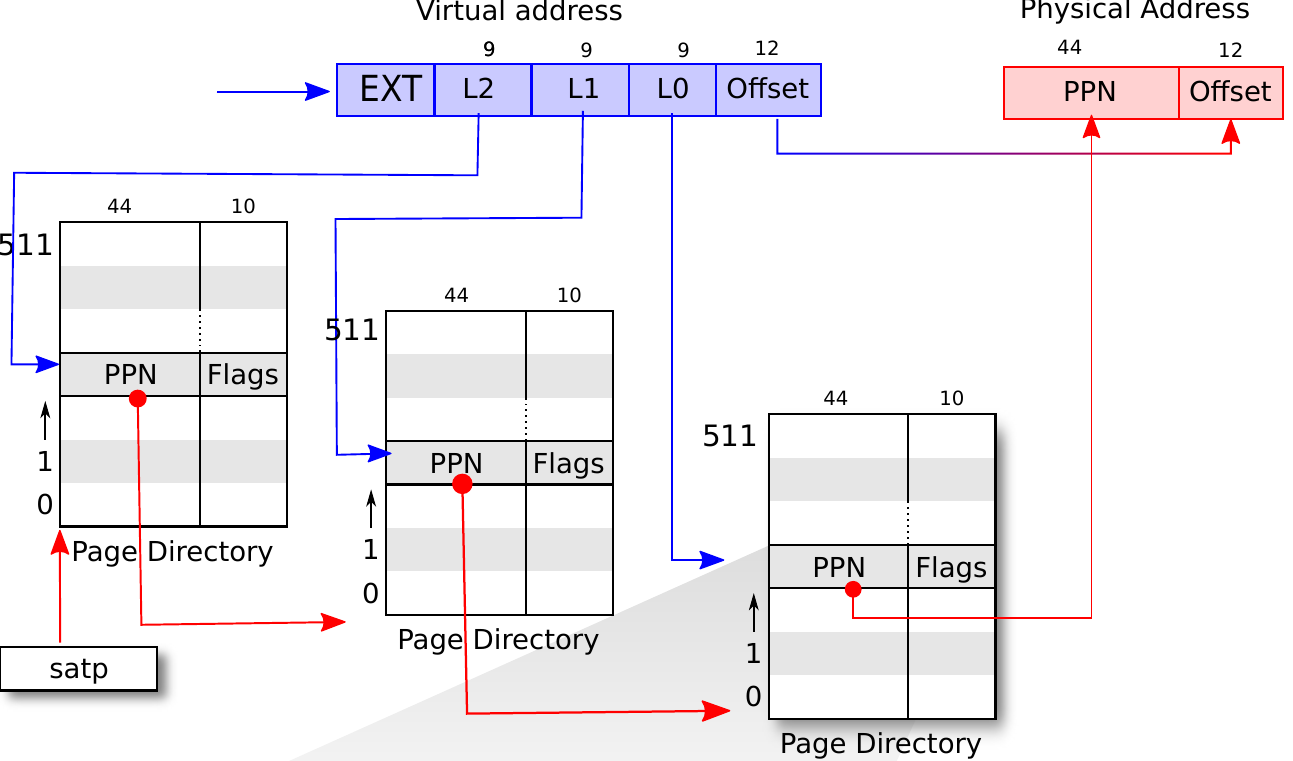
\includegraphics[width=.6\textwidth]{sv39-pagetable}
			
		\end{column}
		
		
		\begin{column}{.5\textwidth}
			
			\begin{itemize}\large
				\item RISC-V对页表的硬件支持
				\begin{itemize}
					\item 页表基址 : satp in RV32/64
					\item  Supervisor Address Translation and Protection (satp) Register
					
					
				\end{itemize}
			\end{itemize}
			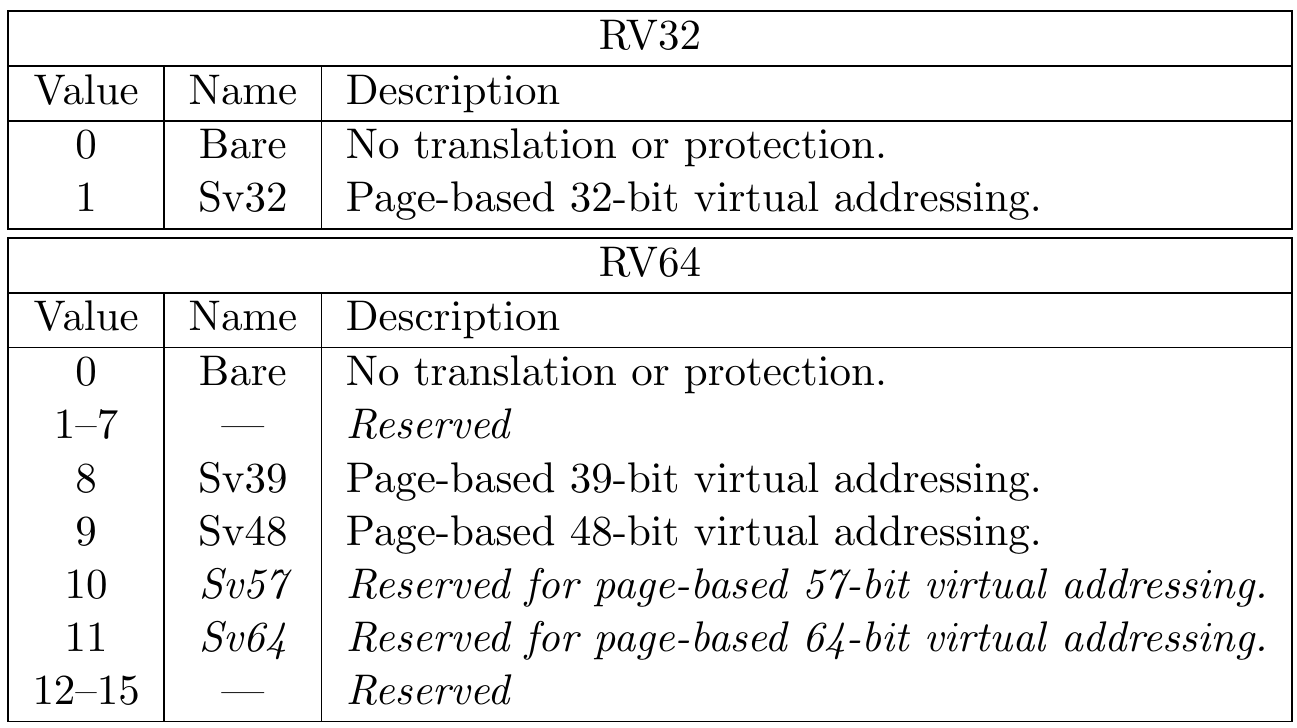
\includegraphics[width=1.\textwidth]{satp-value}
		\end{column}
		
		
	\end{columns}
	
\end{frame}



%------------------------------------------------
\begin{frame}[fragile,plain]   
	\frametitle{RISC-V页映射机制}
	
	\begin{columns}
		
		\begin{column}{.5\textwidth}
			\centering
			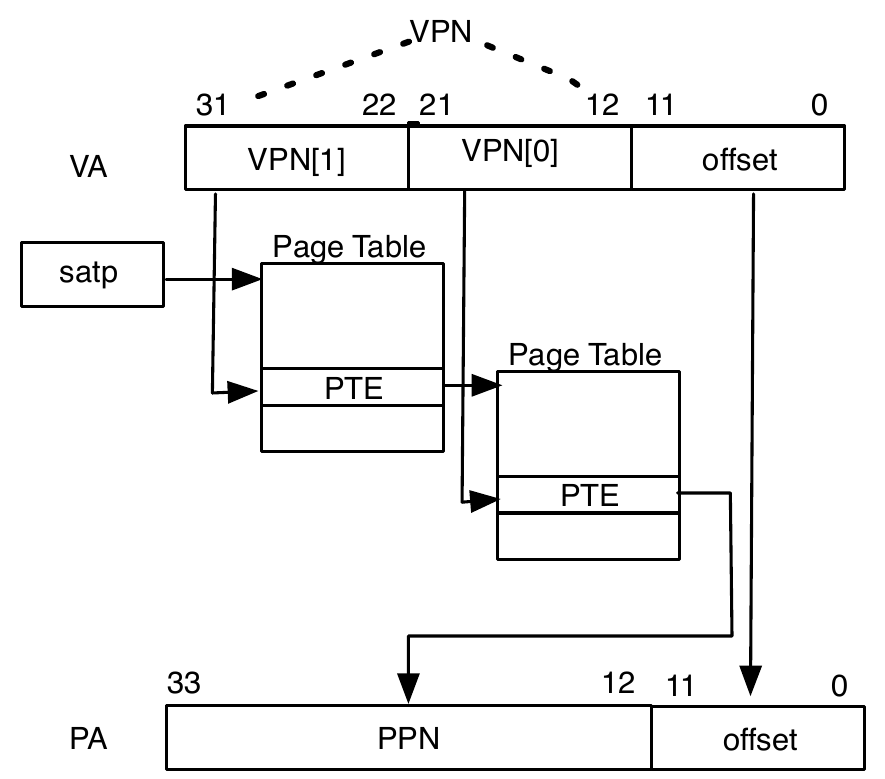
\includegraphics[width=.6\textwidth]{sv32-addr-trans}
			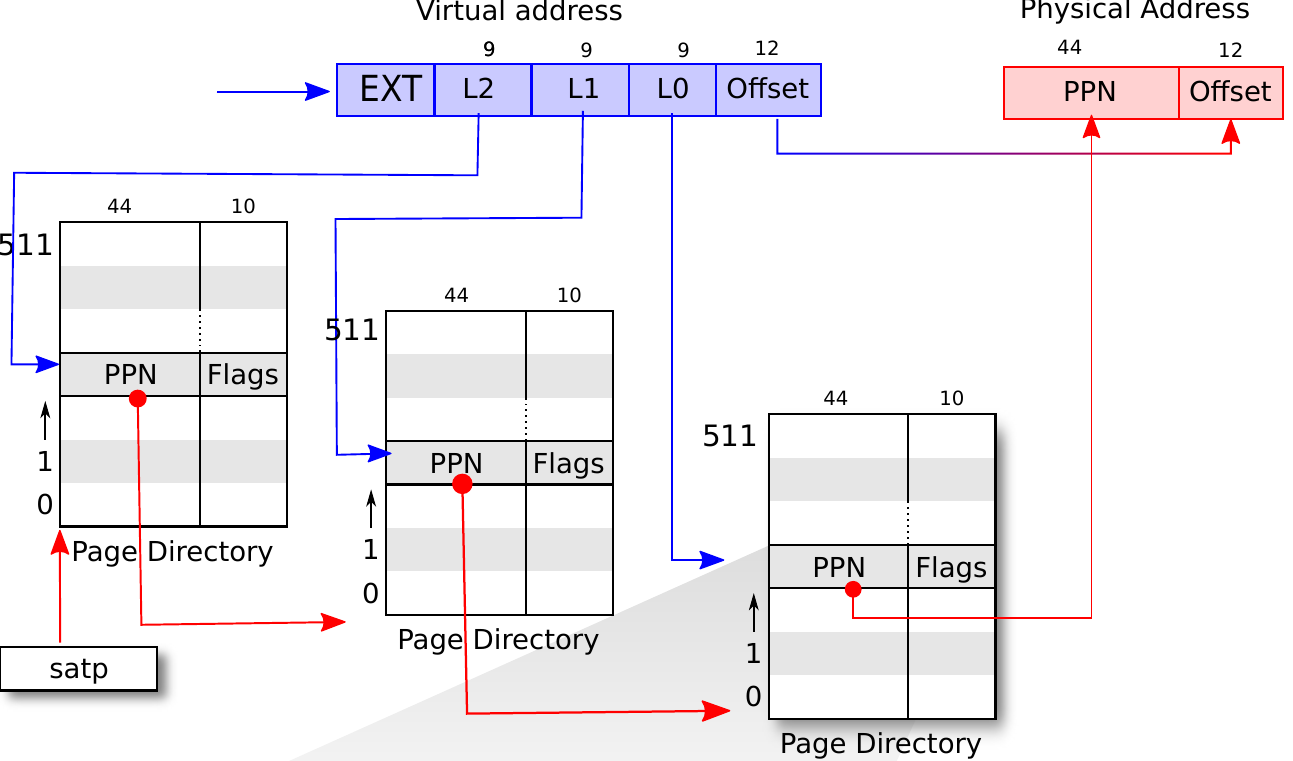
\includegraphics[width=.6\textwidth]{sv39-pagetable}

			
		\end{column}
		
		
		\begin{column}{.5\textwidth}
			
			\begin{itemize}\large
				\item RISC-V对页表的硬件支持
				\begin{itemize}
					\item 地址保护
					\item 页表项(page table entry)
					
					
				\end{itemize}
			\end{itemize}
			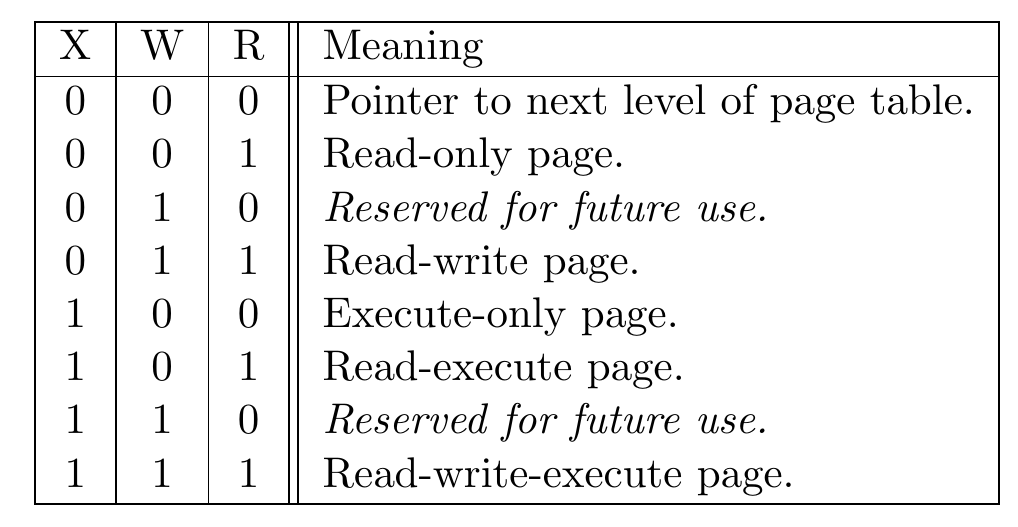
\includegraphics[width=1.\textwidth]{pte-rwx}
		\end{column}
		
%		 R、W 和 X 位分别表示此页是否可以读取、写入和执行。如果这三个位都是 0,
%		那么这个页表项是指向下一级页表的指针,否则它是页表树的一个叶节点。
		
	\end{columns}
	
\end{frame}



%------------------------------------------------
\begin{frame}[fragile,plain]   
	\frametitle{RISC-V页映射机制}
	
	\begin{columns}
		
		\begin{column}{.5\textwidth}
			\centering
			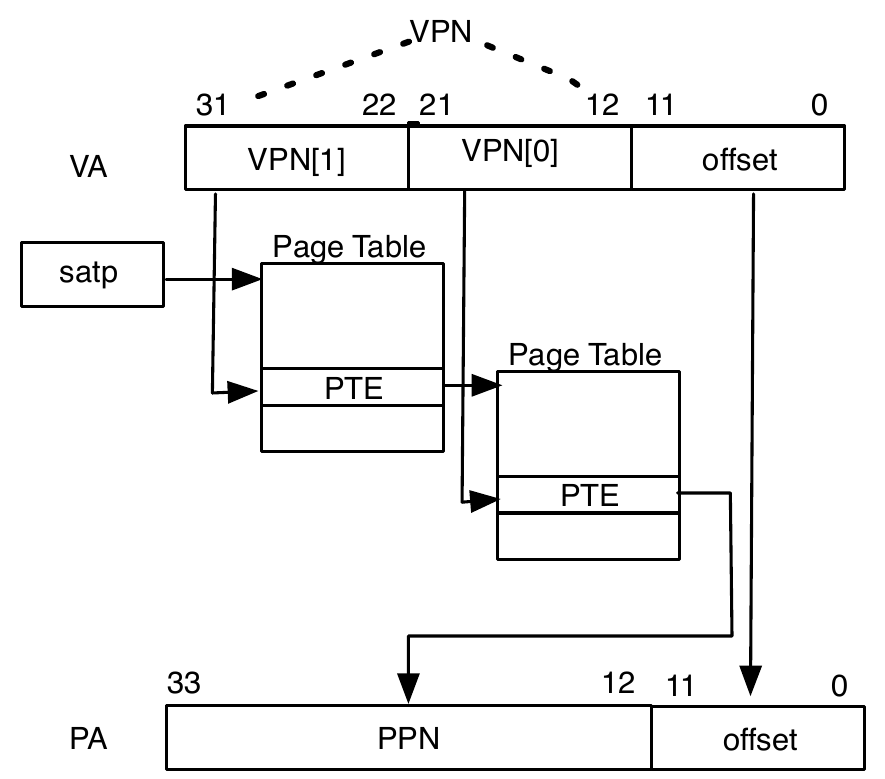
\includegraphics[width=.6\textwidth]{sv32-addr-trans}
			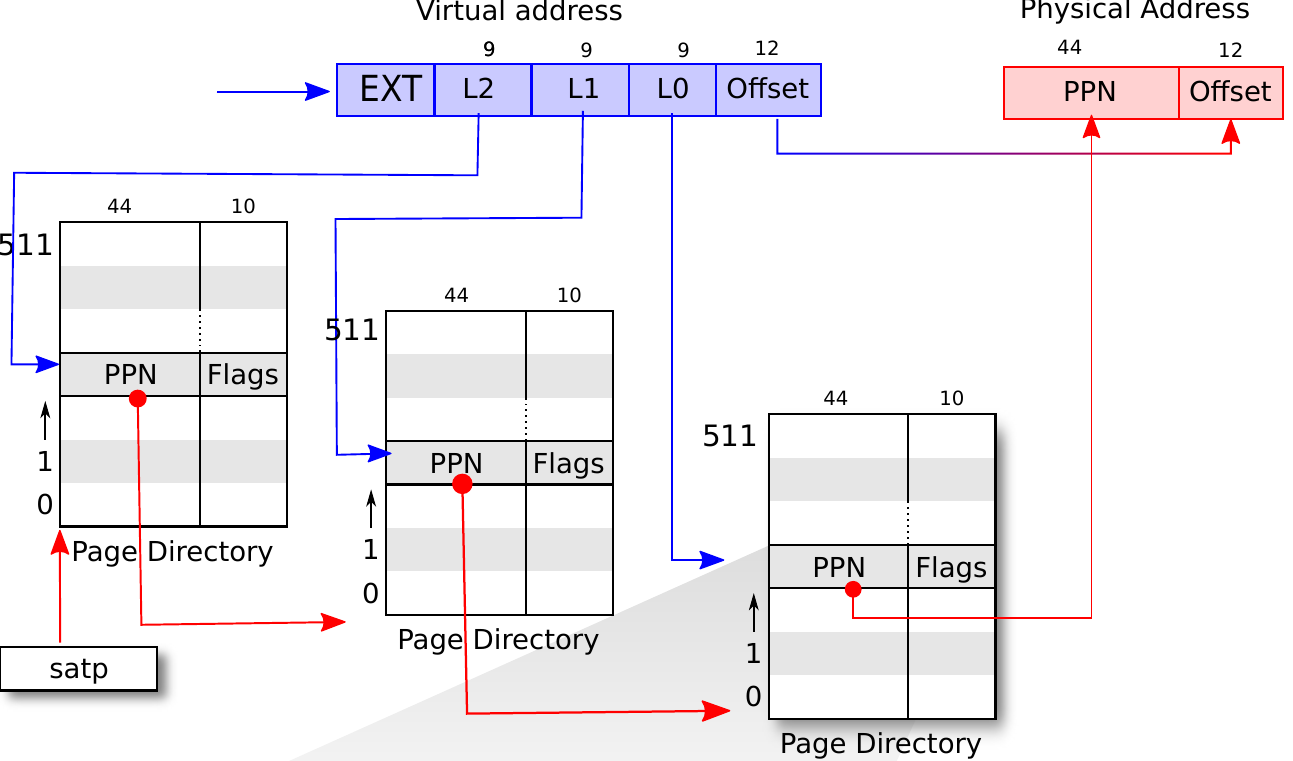
\includegraphics[width=.6\textwidth]{sv39-pagetable}
			
		\end{column}
		
		
		\begin{column}{.5\textwidth}
			
			\begin{itemize}\large
				\item RISC-V对页表的硬件支持
				\begin{itemize}
					\item 地址保护
					\item 页表项(page table entry)
					
					
				\end{itemize}
			\end{itemize}
			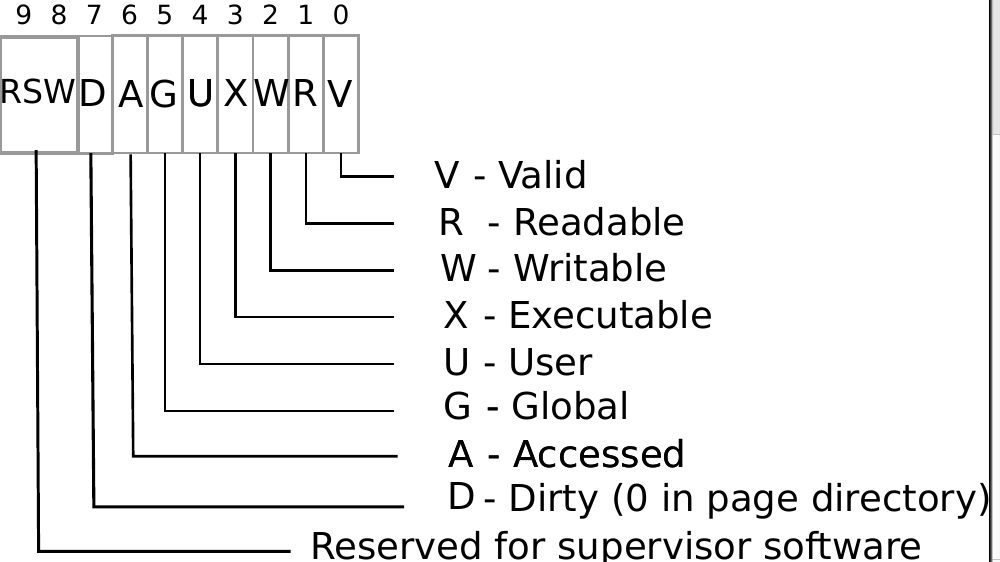
\includegraphics[width=1.\textwidth]{pte-flagbits}
		\end{column}
		
		
	\end{columns}
	
\end{frame}


%------------------------------------------------
\begin{frame}[fragile,plain]   
	\frametitle{RISC-V页映射机制}
	
	\begin{columns}
		
		\begin{column}{.5\textwidth}
			\centering
			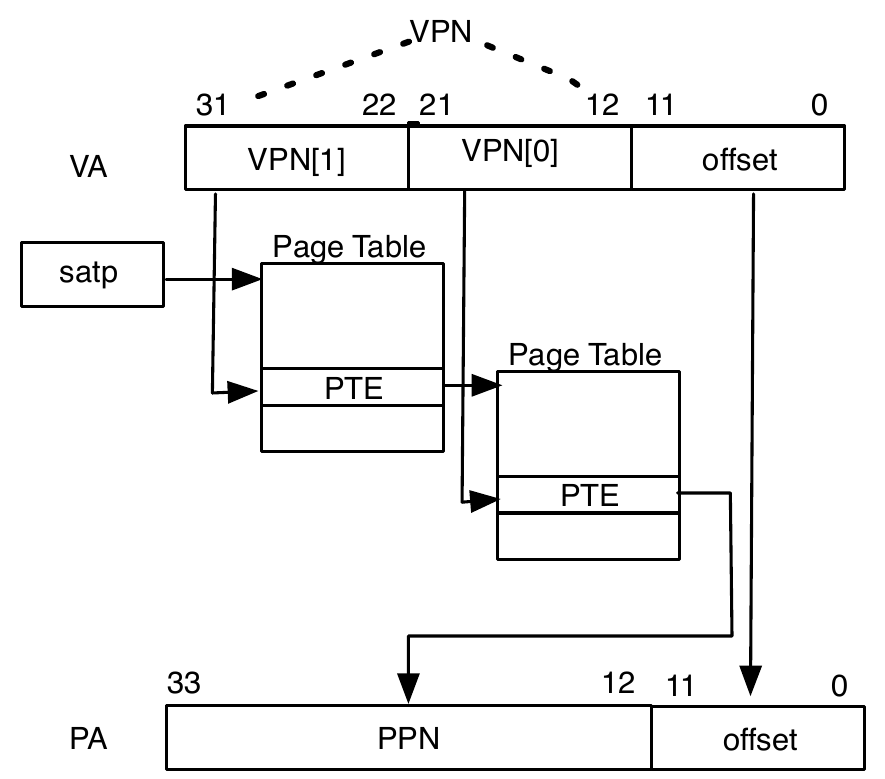
\includegraphics[width=.6\textwidth]{sv32-addr-trans}
			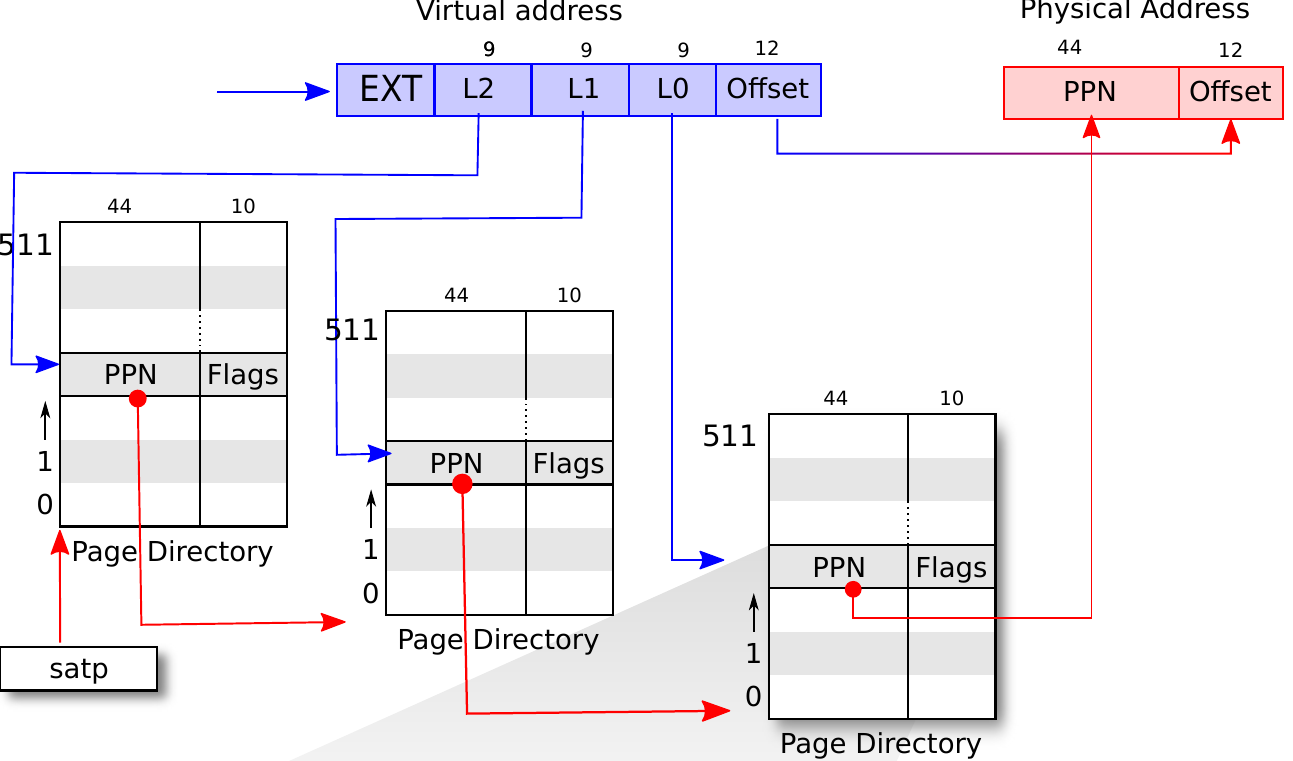
\includegraphics[width=.6\textwidth]{sv39-pagetable}
			
		\end{column}
		
		
		\begin{column}{.5\textwidth}
			
			\begin{itemize}\large
				\item RISC-V对页表的硬件支持
				\begin{itemize}
					\item 地址保护
					\item 页表项(page table entry)
					
%					当在 satp 寄存器中启用了分页时,虚拟地址映射启动。
				\end{itemize}
			\end{itemize}
			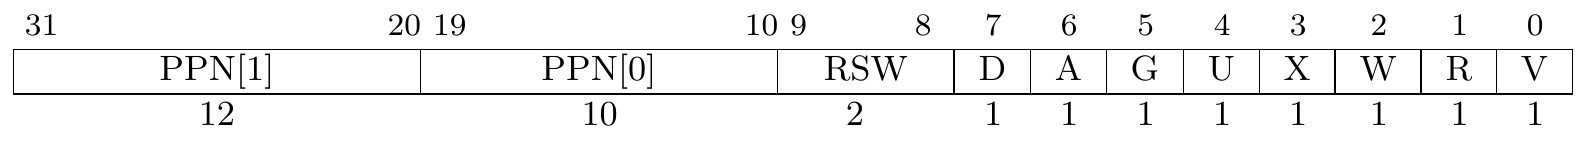
\includegraphics[width=1.7\textwidth]{sv32pte}
			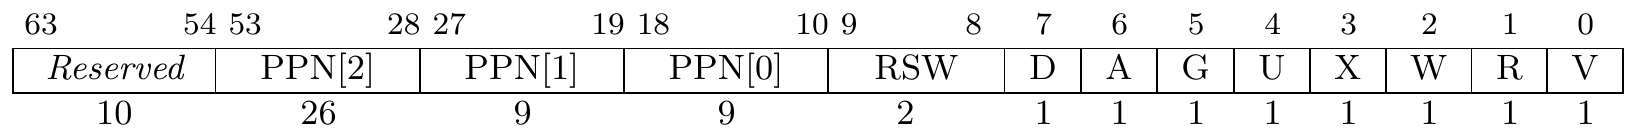
\includegraphics[width=1.7\textwidth]{sv39pte}
%			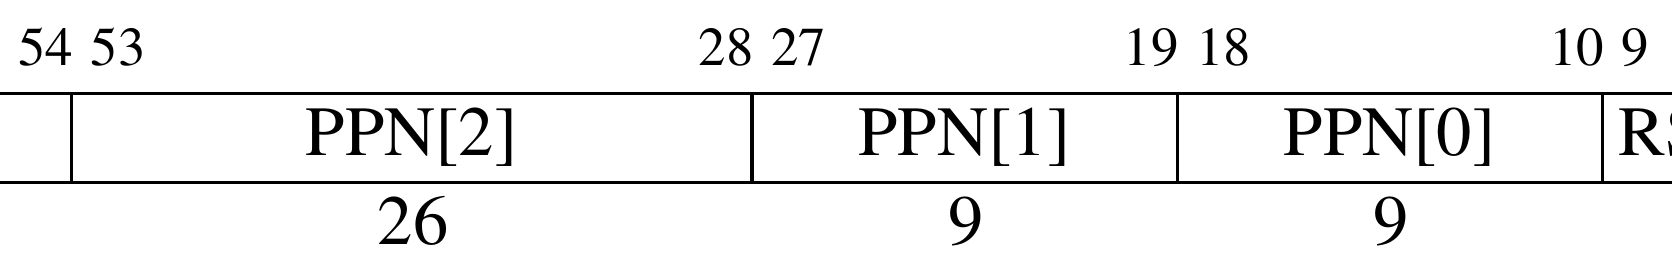
\includegraphics[width=1.\textwidth]{sv39-3ppns}
%			Bits 63–54 are reserved for future use and must be zeroed by software for forward compatibility.

		\end{column}
		
		
	\end{columns}
	
\end{frame}



%------------------------------------------------当在 satp 寄存器中启用了分页时,虚拟地址映射启动。
%\begin{frame}[fragile,plain]   
%	\frametitle{RISC-V页映射机制}
%	
%	\begin{columns}[t]
%		
%		\begin{column}{.5\textwidth}
%			
%			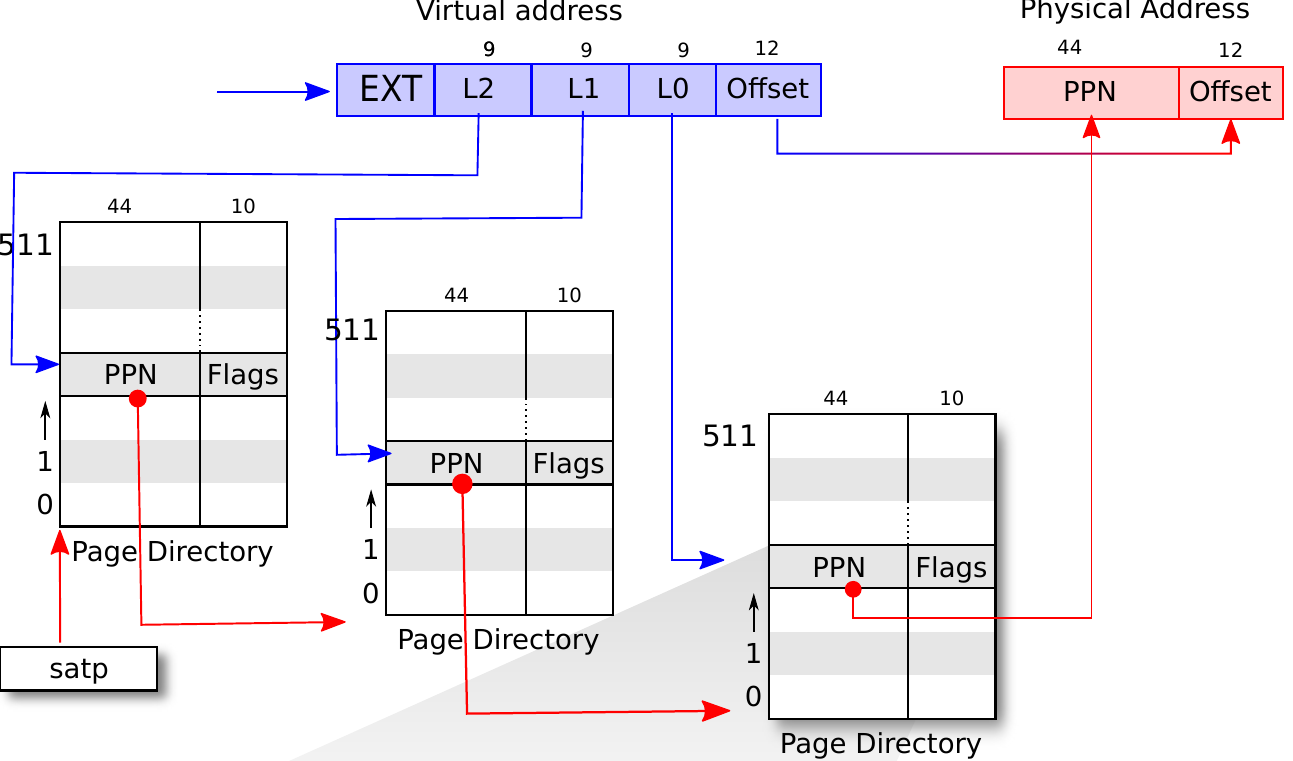
\includegraphics[width=1.\textwidth]{sv39-pagetable}
%			
%		\end{column}
%		
%		
%		\begin{column}{.5\textwidth}
%			
%			\begin{itemize}\large
%				\item RISC-V对页表的硬件支持
%				\begin{itemize}
%					\item 地址保护当在 satp 寄存器中启用了分页时,虚拟地址映射启动。
%					\item 页表项(page table entry)
%					
%					
%				\end{itemize}
%			\end{itemize}
%			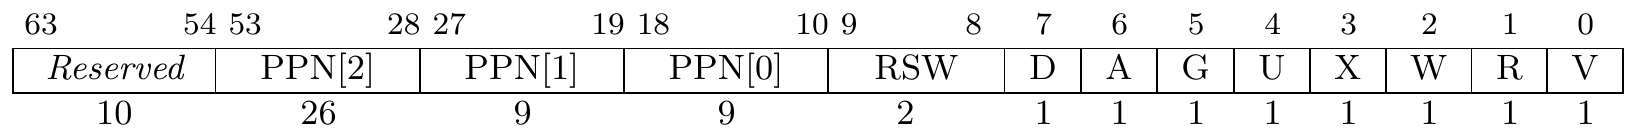
\includegraphics[width=1.\textwidth]{sv39pte}
%			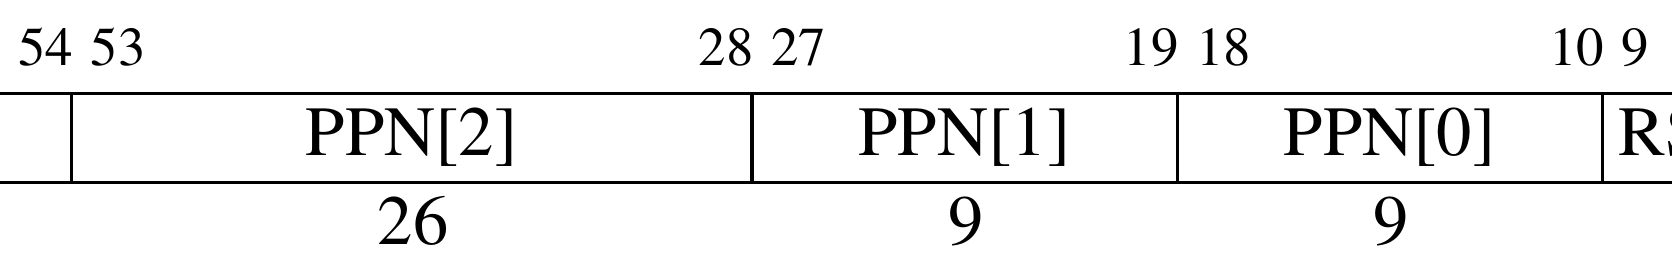
\includegraphics[width=1.\textwidth]{sv39-3ppns}
%%			Bits 63–54 are reserved for future use and must be zeroed by software for forward compatibility.
%%			PPN 域包含物理页号,这是物理地址的一部分。若这个页表项是一个叶节点,那
%%			么 PPN 是转换后物理地址的一部分。否则 PPN 给出下一节页表的地址。
%			
%%Sv39 的 512GiB 地址空间划分为 29 个 1 GiB 大小的吉页。每个吉页被进一步划分为 29 个巨页。在
%%Sv39 中这些巨页大小为 2 MiB,比 Sv32 中略小。每个巨页再进一步分为 29 个 。Sv39 的 512
%%GiB 地址空间划分为 29 个 1 GiB 大小的吉页。每个吉页被进一步划分为 29 个巨页。在
%%Sv39 中这些巨页大小为 2 MiB,比 Sv32 中略小。每个巨页再进一步分为 29 个 4 KiB 大小
%%的基页。4 KiB 大小的基页。
%
%			
%		\end{column}
%		
%		
%	\end{columns}
%	
%\end{frame}
%----------------------------------------------
\subsection{RISC-V地址转换}
\begin{frame}[fragile,plain] 
\frametitle{RISC-V地址转换}

\begin{columns}
	
	\begin{column}{.4\textwidth}
		
		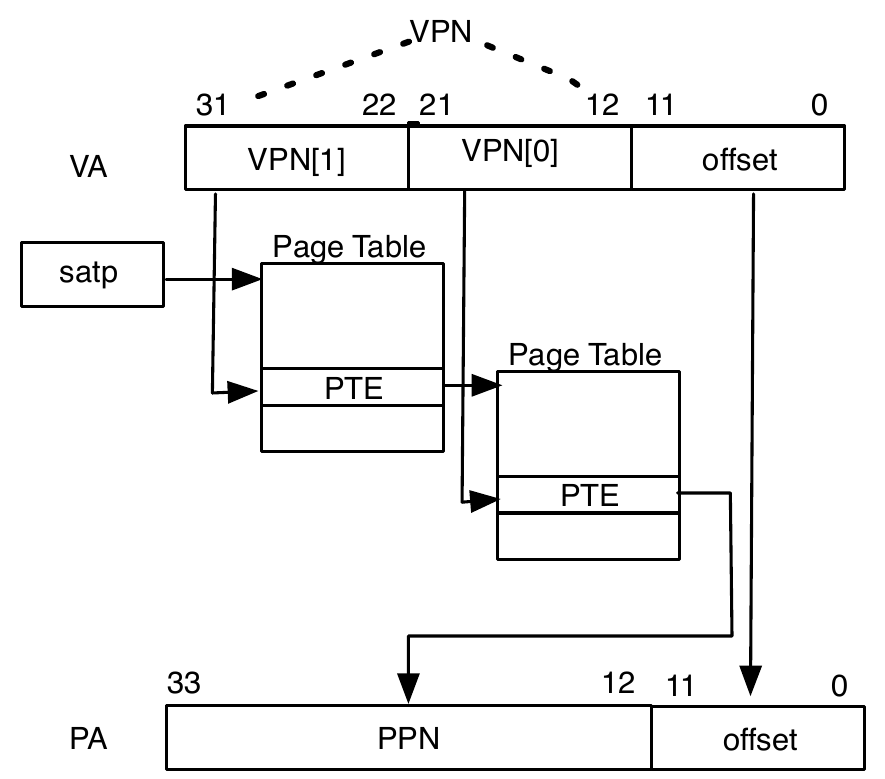
\includegraphics[width=1.\textwidth]{sv32-addr-trans}
		
	\end{column}
	
	
	\begin{column}{.6\textwidth}
		
		\begin{itemize}
			\item Sv32 in RV32
			\begin{itemize}
				\item 当在 satp 寄存器中启用了分页时,虚拟地址映射启动。
				 \item 1. satp.PPN 给出一级页表基址,VA[31:22] VPN[1]给出一级页号,CPU会读取
				位于地址(satp. PPN × 4096 + VA[31: 22] × 4)的页表项。 \pause
				\item 2. 该 PTE 包含二级页表的基址,VA[21:12]给出二级页号,CPU读取位于地
				址(PTE. PPN × 4096 + VA[21: 12] × 4)的叶节点页表项。  \pause
				\item 3. 叶节点页表项的 PPN 字段和页内偏移(原始虚址的最低 12 个有效位)组成了最
				终结果:物理地址就是(LeafPTE. PPN × 4096 + VA[11: 0])
				
%				随后处理器会进行物理内存的访问。Sv39 的转换过程几乎和 Sv32 相同,区别在于其
%				具有较大的 PTE 和更多级页表。
%so in addition to 4 KiB pages, Sv39 supports 2 MiB megapages
%and 1 GiB gigapages, e
			\end{itemize}
		\end{itemize}
		
		
		
	\end{column}
	
	
\end{columns}
\end{frame}

%%----------------------------------------------
%\begin{frame}[fragile,plain] 
%	\frametitle{RISC-V 地址转换}
%	
%	\begin{columns}
%		
%		\begin{column}{1.\textwidth}
%			\centering
%			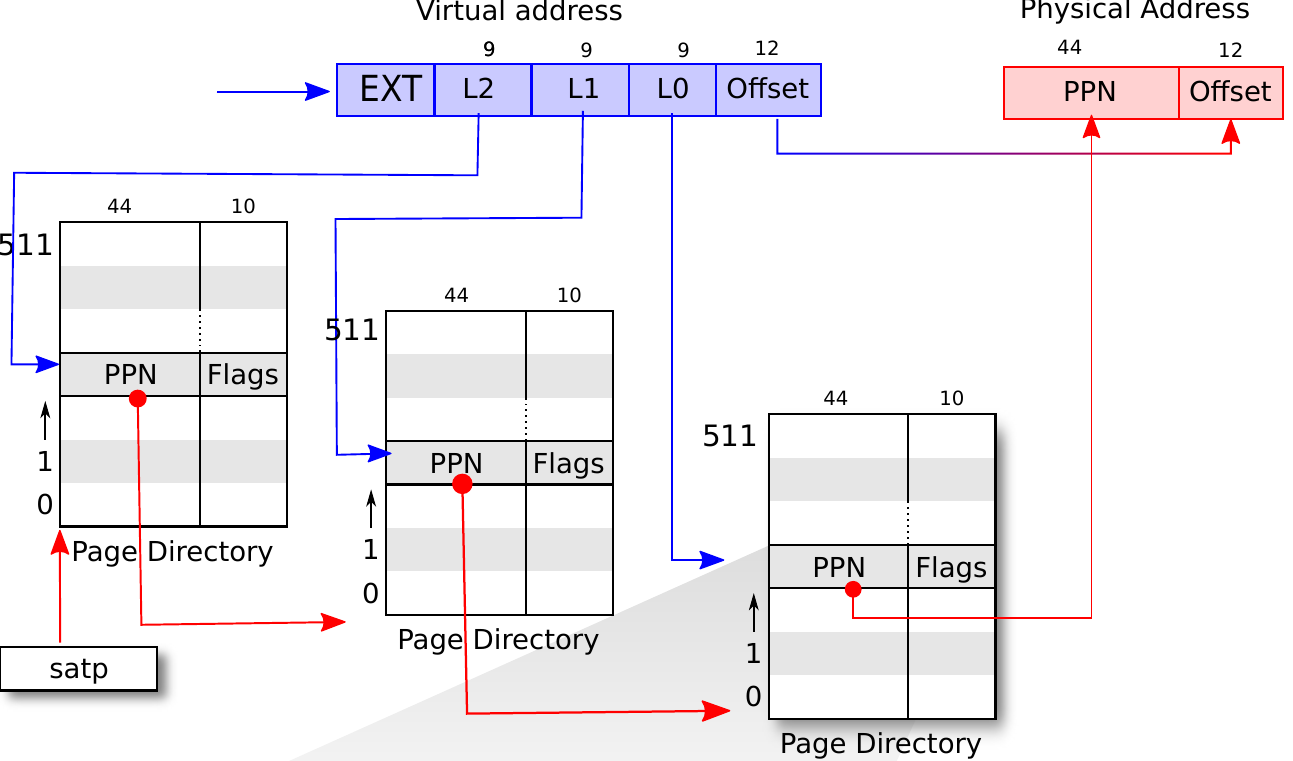
\includegraphics[width=.8\textwidth]{sv39-pagetable}
%			
%		\end{column}
%		
%		
%		\begin{column}{.1\textwidth}
%			
%			%			\begin{itemize}\Large
%			%%				\item 
%			%				\begin{itemize}\large
%			%%					\item 
%			%					
%			%				\end{itemize}
%			%			\end{itemize}
%			
%		\end{column}
%		
%		
%	\end{columns}
%\end{frame}


%----------------------------------------------
\begin{frame}[fragile,plain] 
	\frametitle{RISC-V 地址转换}
	
	\begin{columns}
		
		\begin{column}{.4\textwidth}
			
			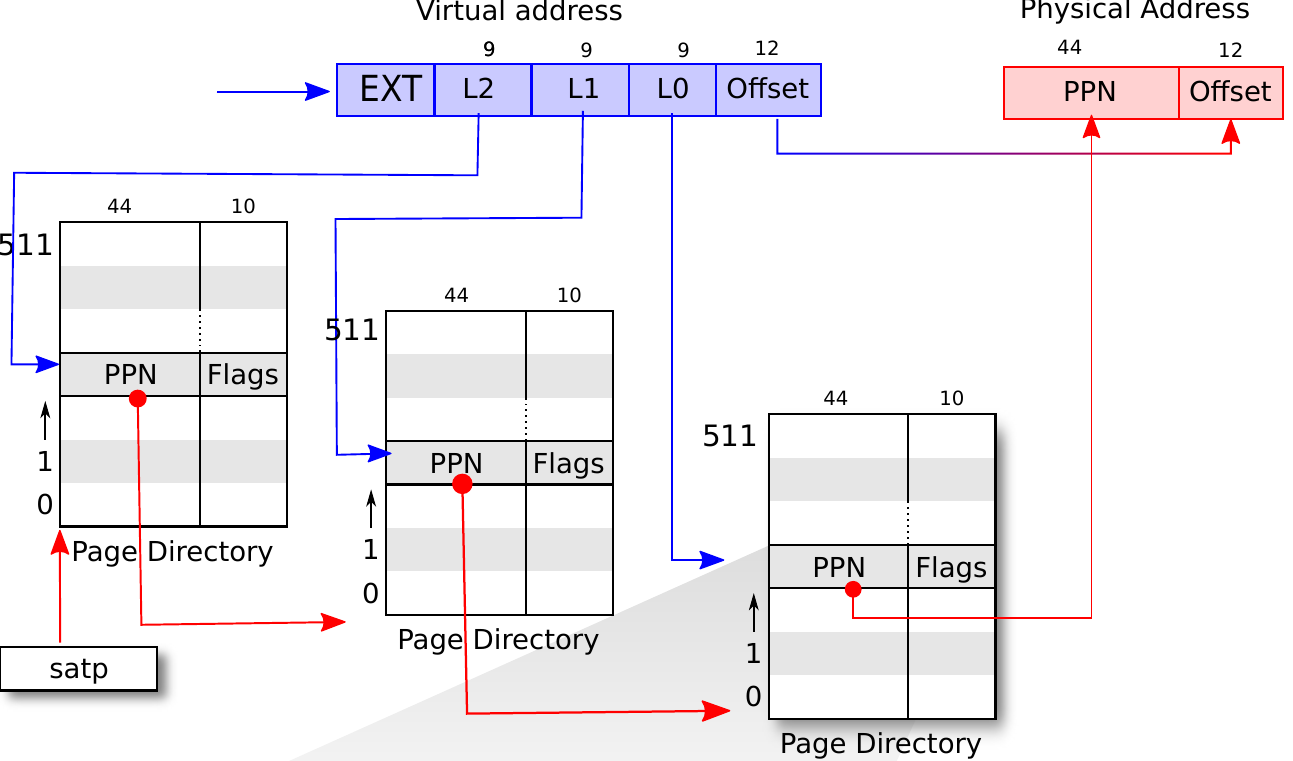
\includegraphics[width=1.2\textwidth]{sv39-pagetable}
			
		\end{column}
		
		
		\begin{column}{.6\textwidth}
			
			\begin{itemize}
				\item Sv39 in RV64 
				\begin{itemize}\small
				 	\item 地址映射要计算三次
					\item (satp.PPN × 4K + L2 × 8)的页目录项
					\item (PTE.PPN × 4K + L1 × 8)的二级页目录项
					\item (LeafPTE.PPN × 4K +L0 x 8)叶节点页表项
					\item 叶节点页表项的PPN 字段 × 4K + Offset
					
					%				随后处理器会进行物理内存的访问。Sv39 的转换过程几乎和 Sv32 相同,区别在于其
					%				具有较大的 PTE 和更多级页表。
					%so in addition to 4 KiB pages, Sv39 supports 2 MiB megapages
					%and 1 GiB gigapages, e
				\end{itemize}
			\end{itemize}
			
			
			
		\end{column}
		
		
	\end{columns}
\end{frame}


%----------------------------------------------
\end{document}
